\documentclass[xcolor=dvipsnames]{beamer} 
\usecolortheme[named=Blue]{structure} 
\usetheme[height=10.5mm]{Rochester} 
\setbeamertemplate{items}[ball] 
\setbeamertemplate{blocks}[rounded][shadow=true] 
\setbeamertemplate{navigation symbols}{} 
\usepackage{bm}
\usepackage{listings}
\usepackage{rotating}
\usepackage{graphicx}
\usepackage{multirow}
\usepackage{hyperref}
\usepackage{textcomp}
\usepackage{upquote}
\usepackage[absolute,overlay]{textpos}
\newenvironment{reference}[2]{%
  \begin{textblock*}{\textwidth}(#1,#2)
      \footnotesize\it\bgroup\color{red!50!black}}{\egroup\end{textblock*}}
%\graphicspath{ {/home/ben/PhD/Armidale_Updates/2014_03_14/Figures/} }
\begin{document}

%%% New plan for this module:
%%% we all use Git on the command line and view GitHub in our web browsers
%%% clone and commit via HTTPS
%%% Workflow plan:
%%%
%%% Create repo in web browser
%%% Authenticate on cmd line
%%% Clone
%%% Add files
%%% Edit
%%% git add
%%% git commit
%%% branch and revert to previous version with check out


%%% Getting on the command line in various OS's

%%% MS Windows -> Start Menue -> Powershell
%%% Mac OS -> Finder -> terminal
%%% GNU+Linux users -> application launcher (will vary depending on GUI) -> terminal 


\begin{frame} %1
% \frametitle{Addressing Common Challenges in Spatial Modeling of Ecologies and Environments}
\begin{center}
\textbf{\huge Installing Git on MacOS}\\
\end{center}

\begin{figure}
%\includegraphics[width = 0.35\textwidth]{/home/ben/Intro_to_R/GitHub_Slides_Source/Images/GitHub-Mark-120px-plus.png}
\begin{columns}

\begin{column}{3.3cm}
\begin{center}
\begin{figure}

\includegraphics[width = 0.9\textwidth]{/home/ben/Intro_to_R/Introductory_Slides_Source/Images/R_logo.png}
\end{figure}
\end{center}
\end{column} 

\begin{column}{3.3cm}
\begin{center}
\begin{figure}

\includegraphics[width = 0.9\textwidth]{/home/ben/Intro_to_R/GitHub_Slides_Source/Images/Git-Icon-1788C.pdf}
\end{figure}
\end{center}
\end{column} 

\begin{column}{3.3cm}
\begin{center}
\begin{figure}

\includegraphics[width = 0.9\textwidth]{/home/ben/Intro_to_R/GitHub_Slides_Source/Images/GitHub-Mark_Big.pdf}
\end{figure}
\end{center}
\end{column} 

\end{columns}
\end{figure}

\small Ben R. Fitzpatrick\\
\tiny PhD Candidate, Statistical Science, Mathematical Sciences School, Queensland University of Technology
\newline
\begin{columns}
\begin{column}{3cm}
\tiny 0000-0003-1916-0939
\end{column}
\begin{column}{3cm}
\tiny github.com/brfitzpatrick/
\end{column}
\begin{column}{3cm}
\tiny @benrfitzpatrick
\end{column}
\end{columns}
\end{frame}

\begin{frame}
\frametitle{Download Git}
\framesubtitle{\url{http://git-scm.com/downloads}}
\begin{center}
\begin{figure}
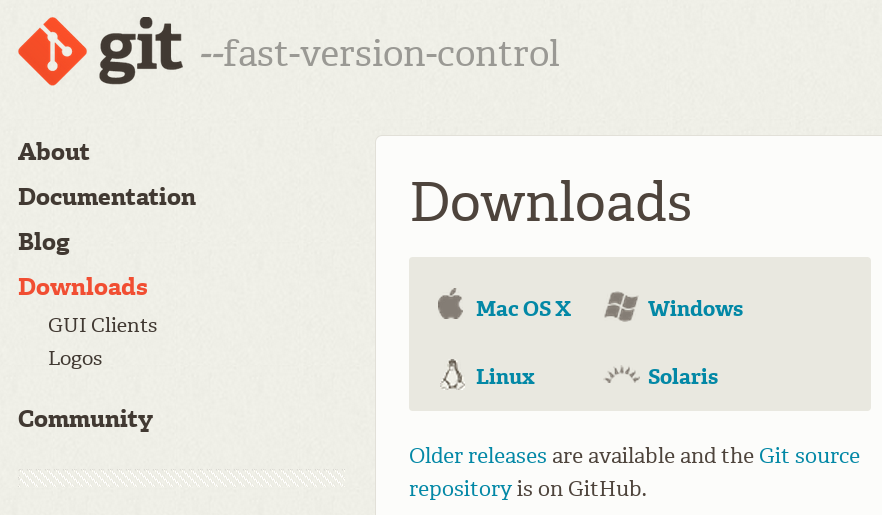
\includegraphics[width = \textwidth]{/home/ben/Tests/Git_MacOS_Install/Download_Git.png}
\end{figure}
\end{center}
\end{frame}


\begin{frame}
\frametitle{Step 1}
\begin{center}
\begin{figure}
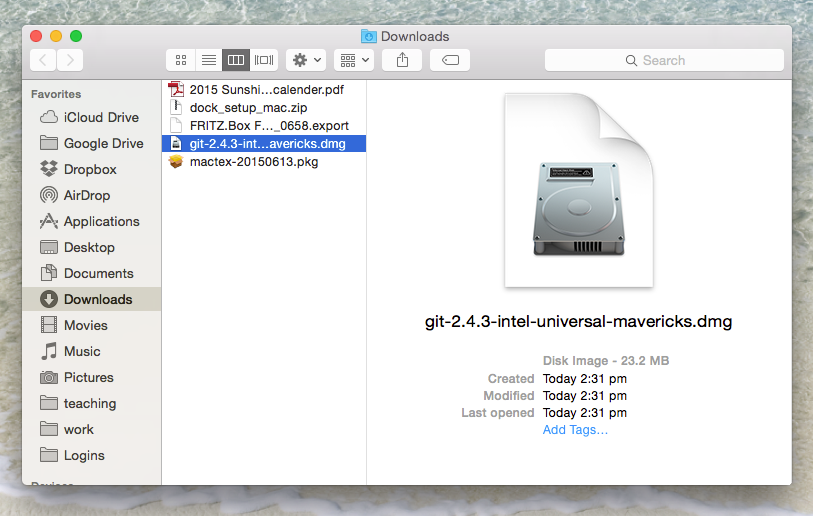
\includegraphics[width = \textwidth]{/home/ben/Tests/Git_MacOS_Install/GI_OSX_1.png}
\end{figure}
\end{center}
\end{frame}

\begin{frame}
\frametitle{Step 2}
\begin{center}
\begin{figure}
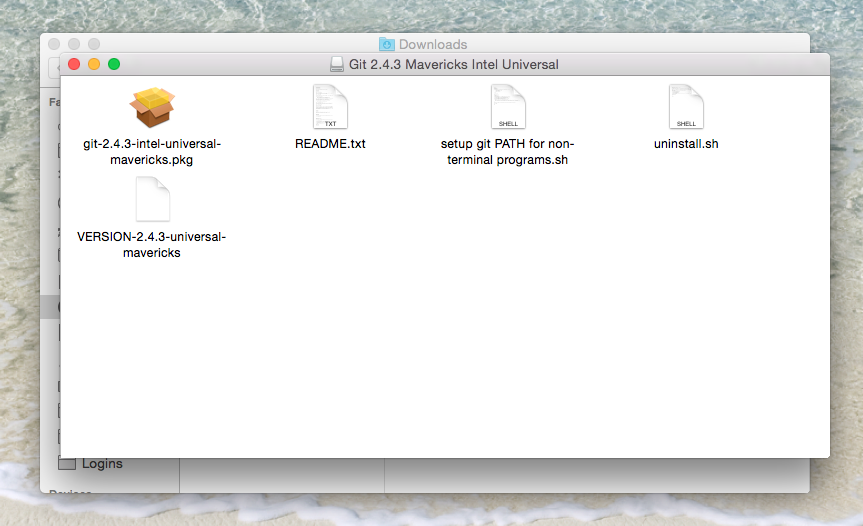
\includegraphics[width = \textwidth]{/home/ben/Tests/Git_MacOS_Install/GI_OSX_2.png}
\end{figure}
\end{center}
\end{frame}

\begin{frame}
\frametitle{Step 3}
\begin{center}
\begin{figure}
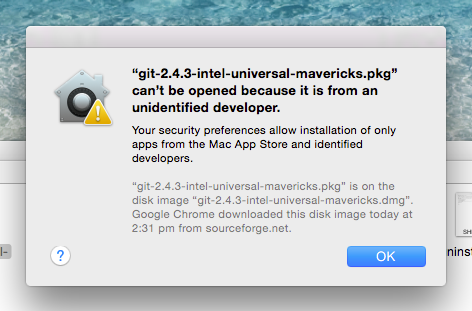
\includegraphics[width = \textwidth]{/home/ben/Tests/Git_MacOS_Install/GI_OSX_3.png}
\end{figure}
\end{center}
\end{frame}


\begin{frame}
\frametitle{Step 4}
\framesubtitle{You may need to relax your security setting briefly}
If this makes you uncomfortable you're welcome to watch the session rather than participating
\begin{center}
\begin{figure}
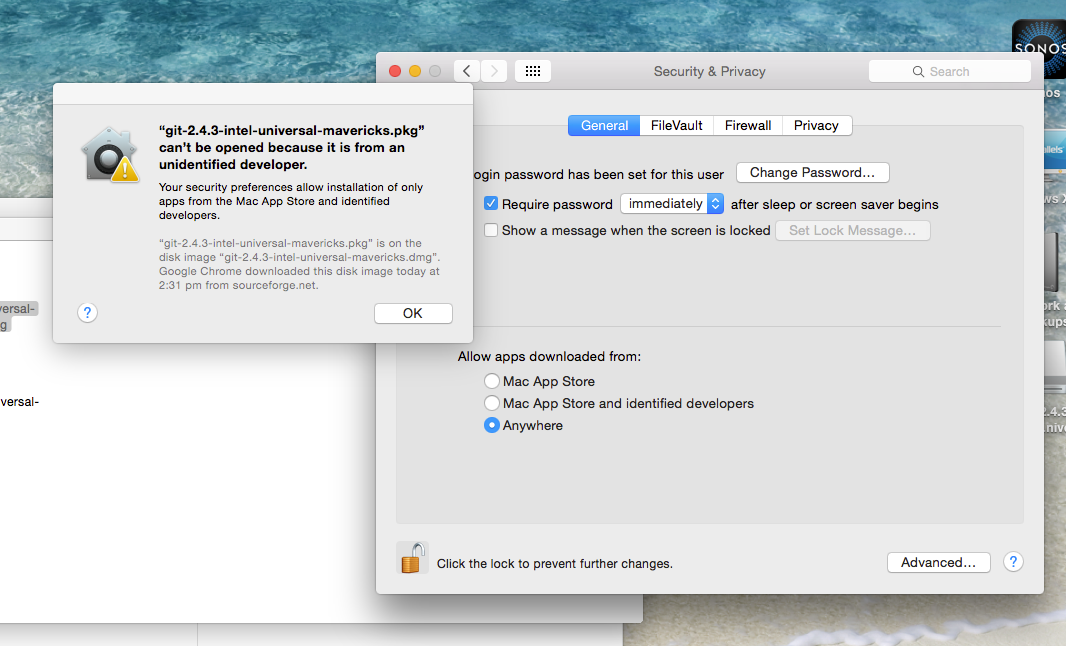
\includegraphics[width = \textwidth]{/home/ben/Tests/Git_MacOS_Install/GI_OSX_4.png}
\end{figure}
\end{center}
\end{frame}


\begin{frame}
\frametitle{Step 5}
\begin{center}
\begin{figure}
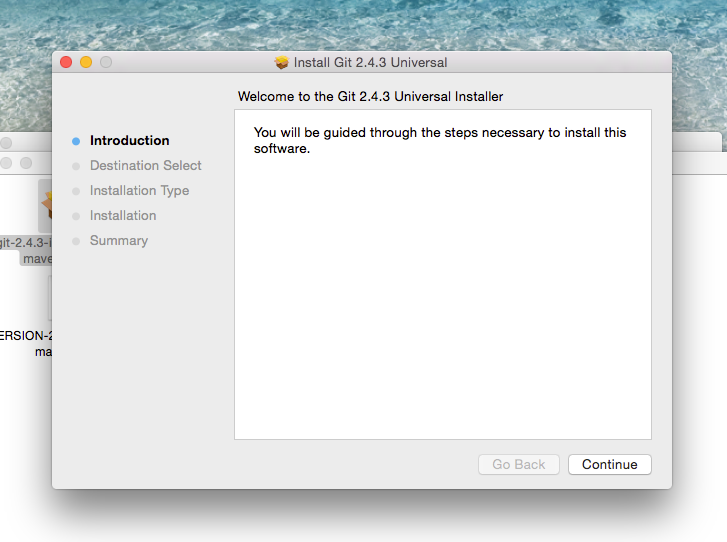
\includegraphics[width = \textwidth]{/home/ben/Tests/Git_MacOS_Install/GI_OSX_5.png}
\end{figure}
\end{center}
\end{frame}

\begin{frame}
\frametitle{Step 6}
\begin{center}
\begin{figure}
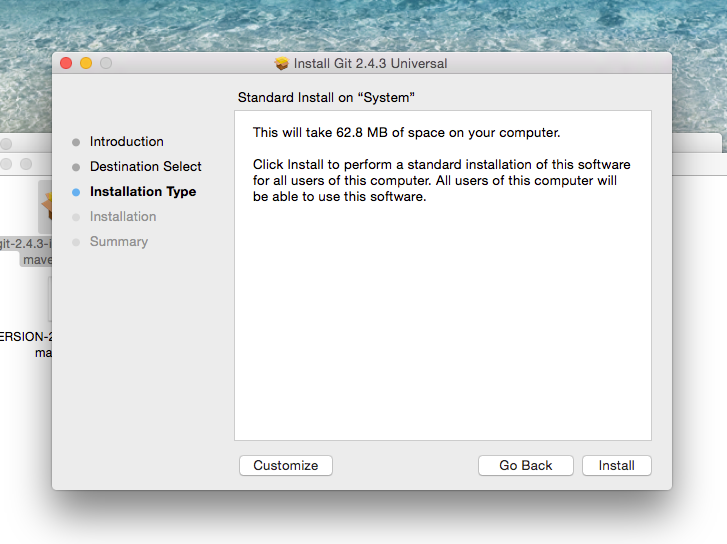
\includegraphics[width = \textwidth]{/home/ben/Tests/Git_MacOS_Install/GI_OSX_6.png}
\end{figure}
\end{center}
\end{frame}

\begin{frame}
\frametitle{Step 7}
\begin{center}
\begin{figure}
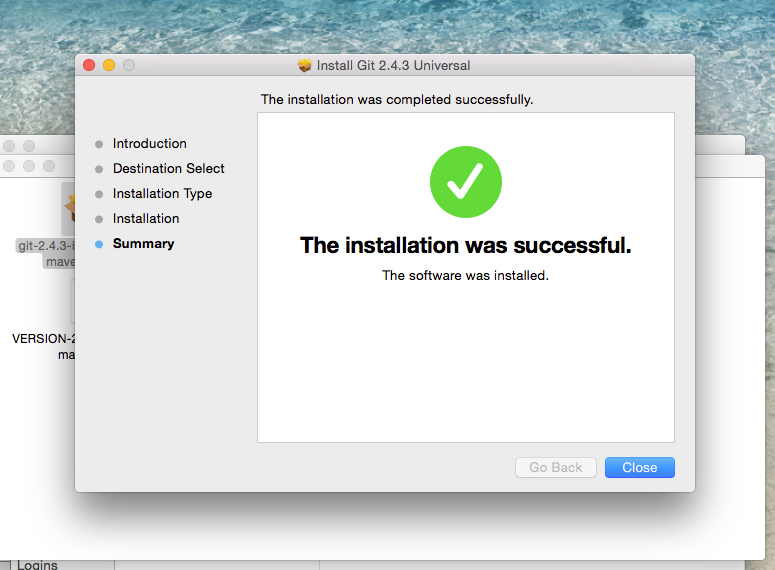
\includegraphics[width = \textwidth]{/home/ben/Tests/Git_MacOS_Install/GI_OSX_7.png}
\end{figure}
\end{center}
\end{frame}

\begin{frame}
\frametitle{Step 8}
\framesubtitle{Check Git is installed:}
\begin{center}
\begin{figure}
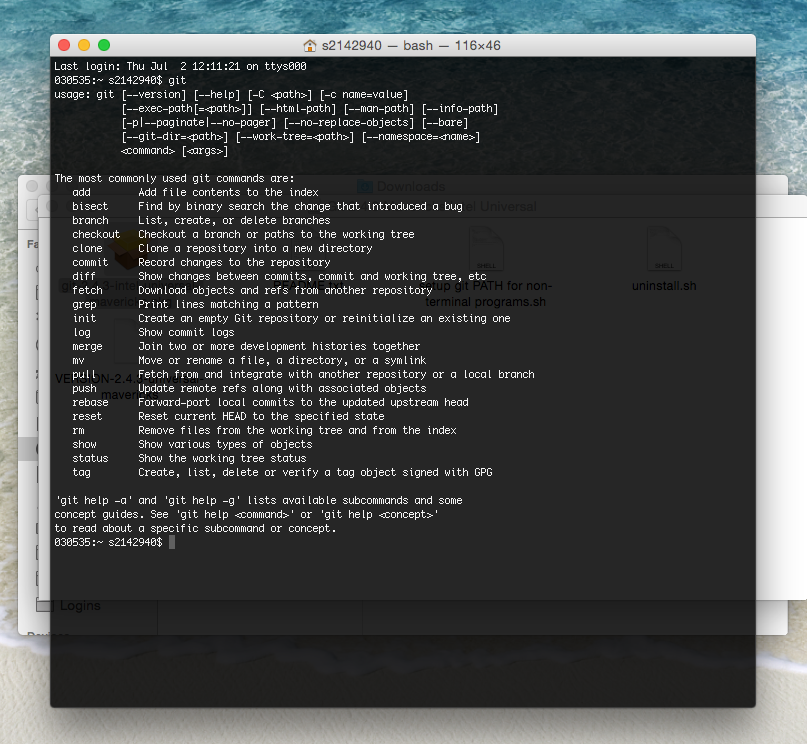
\includegraphics[height = 0.9\textheight]{/home/ben/Tests/Git_MacOS_Install/GI_OSX_8.png}
\end{figure}
\end{center}
\end{frame}




\end{document}
